\chapter{Background}\label{sec:Background}
RL is a process that requires both interactive parts as well as algorithms that improve interactions. The following section \ref{reinforcement_learning} introduces the general concept of RL and its specifications. Afterwards, two popular learning algorithms for RL problems are presented: PPO and DQN.

\section{Reinforcement Learning}\label{reinforcement_learning}
Sutton and Barto wrote in ``Reinforcement learning: An introduction'' \cite{suba18} that RL is based on two components that interact with each other: an environment and an agent, see Figure \ref{fig:rl_cycle}. Those interactions take part during a time period with discrete time steps $t\in\mathbb{N}_0$ until a goal is reached or the ending condition applies. This process is called an episode. Formally, the journey of the agent to find the goal is described as a Markov Decision Process (MDP) \cite{suba18}. When multiple agents act in the same environment, the Markov decision process is called a stochastic game \cite{buba10}.

\begin{figure}[hpbt]
    \centering
    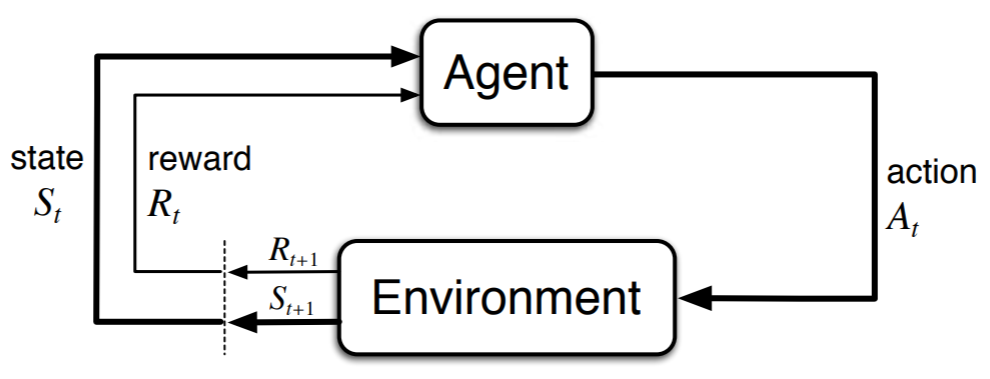
\includegraphics[width=0.6\textwidth]{pictures/RLInteractionSB}\\
    \caption[Reinforcement Learning Cycle]{The cycle of agent-environment interaction as
        shown in ``Reinforcement learning: An introduction'' \cite{suba18}}\label{fig:rl_cycle}
\end{figure}

One environment state $S_t$ is part of a set $S$ containing all possible states. In most cases, the environment state describes what the agent can see. An agent often only has a small field of view, which turns a MDP into a partially observable MDP \cite{suba18}. During each point in time $t$, the agent can interact with the environment by executing an action $A_t$, which changes the environment state. An example would be moving in the environment, which results in a new area that the agent can now see. In a multiagent environment, every agent chooses its action simultaneously and adds it into a joint action set, which is executed collectively during $t$ \cite{buba10}.

The reward $R_t$ is an element of a set of possible rewards $R \subset \mathbb{R}$ \cite{suba18}. Therefore, the reward can potentially be negative. Depending on the environment, that value can act as immediate feedback to the agents action. Other times, the reward is received as a result of a whole action sequence or the achievement of a certain state, for instance the goal or subgoals. The general concept of RL, as defined by Sutton and Barto \cite{suba18}, is for agents to maximize rewards. Unlike machine learning approaches, the agent starts with no knowledge about good or bad actions and enhances the decision-making over time.

Sutton and Barto defines the agents' action selection with respect to the current state as a policy $\pi$. They explain further that a policy could be as simple as a lookup table, mapping states to actions, or it could contain a complicated search process for the best decision. However, policies most of the time map action-state pairs to a selection probability, with all actions of a state adding up to 100\%.
During environment interactions, agents receive rewards which can be used to update the policy accordingly. As an example, the probability of policy $\pi(a \mid s)$ decreases when receiving a negative or low reward, reducing the chances of executing the same action in that specific state again.

While rewards only rate the immediate situation, a value function, i.e. the state-value function $V^\pi(s_t)$ for a policy $\pi$, can be used to estimate the long-term value of a state $s$ \cite{suba18}:
\begin{equation}\label{eq:value_func}
    v_\pi(s) \doteq \mathbb{E}_\pi \left[ G_t \mid S_t = s \right] = \mathbb{E}_\pi \left[ \sum^{\infty}_{k=0} \gamma^k R_{t+k+1 \mid S_t = s}  \right]
\end{equation}
The result is the estimated discounted cumulative reward an agent could get following that state and choosing actions based on the current policy. The discount factor is defined by Sutton and Barto as $0 \le \gamma < 1$ and provides a constant that reduces the importance of future rewards. A high $\gamma$ symbolizes a greater interest in rewards that are far away, whereas a discount of zero only takes the current reward into account. By setting $\gamma$ smaller than one, it is ensured that the infinite sum results in a value. Generally, states that offer immediate high rewards could end in a low reward streak. In the opposite case, a low reward state could subsequently yield high rewards. Therefore, value functions are of great use to achieve the maximum reward.

The last part to note about RL is that it entails the problem of balancing exploration and exploitation \cite{suba18}. On the one hand, an agent has to explore different options in order to learn and expand its knowledge. On the other hand, agents strive to maximize the reward, which can lead to greediness. An agent could start to exploit its knowledge too early, choosing actions of which it knows to result in positive rewards. However, if an agent does not explore enough, the best action sequence will stay hidden and the agents knowledge will not improve.

\section{Proximal Policy Optimization}
In 2017, Schulman et al. introduced the concept of PPO in the article ``Proximal Policy Optimization Algorithms'' \cite{scwo17}. Policy optimization is the improvement of the action selection strategy $\pi$ based on the current state $s_{t}$. This is achieved by rotating two steps \cite{scwo17}: \\
\begin{enumerate}
  \item Sampling data from the policy and
  \item Optimizing the objective with that data through several epochs.
\end{enumerate}

Using those steps results in the agent gathering a small batch of experiences while choosing actions with a policy $\pi$. Afterwards, this batch is used once to enhance the current policy. Then, the experiences are discarded and the agent uses the updated policy to gather a new batch. By repeating those two steps the agent can learn to choose better actions. PPO is applied to prevent drastic policy changes, which stabilizes the learning process.

The origin of PPO lies in a similar approach called Trust Region Policy Optimization (TRPO). TRPO also restricts policy updates by defining a trust region \cite{scle15}. This is achieved by maximizing the following function \cite{scwo17}:
\begin{equation}\label{eq:TRPO}
    \underset{\theta}{maximize}\,\hat{\mathbb{E}}_{t} \left[ \frac{\pi_{\theta}(a_{t} \mid s_{t})}{\pi_{\theta_{old}}(a_{t} \mid s_{t})}
        \hat{A}_{t}-\beta \, KL[\pi_{\theta_{old}}(\cdot \mid s_{t}),\pi_{\theta}(\cdot \mid s_{t})] \right]
\end{equation}
The expectation $\hat{\mathbb{E}}_{t}$ indicates, that an empirical average over a number $t$ of samples is used for estimation and the algorithm alternates between sampling and executing these calculations. The variable $\hat{A}_{t}$ describes an estimator of the advantage function. This function was defined in the paper ``Trust Region Policy Optimization'' \cite{scle15} with \\ $A_\pi(s,a) = Q_\pi(s,a)-V_\pi(s)$. The first part calculates the state-action value, estimating the upcoming rewards for an agent, starting at state s and initially selecting action a. Afterwards, the action selection is based on the current policy $\pi$. 

The second part contains the state value function $V_\pi(s)$, which works very similarly by starting at state s and using $\pi$. However, the difference is that the agent always chooses actions according to the policy. The result of the advantage function $A_\pi(s,a)$ shows whether a profit could be gained when deviating from the policy by specifically choosing action a.

The fraction $\frac{\pi_{\theta}(a_{t} \mid s_{t})}{\pi_{\theta_{old}}(a_{t} \mid s_{t})}$ in the Minuend of function \eqref{eq:TRPO} can be replaced by $r(\theta)$
and represents the probability ratio of an action in the current policy in comparison to the old policy \cite{scwo17}. $\theta$ represents a policy parameter. The result of $r(\theta)$ is greater than one, if an action is very probable in the current policy. Otherwise, the outcome lies between zero and one. Schulman et al. \cite{scwo17} further extract the first part of function \eqref{eq:TRPO} as the surrogate objective:
\begin{equation}\label{eq:TRPO_surrogate}
    L^{CPI}(\theta) = \hat{\mathbb{E}}_{t} \left[ \frac{\pi_{\theta}(a_{t} \mid s_{t})}{\pi_{\theta_{old}}(a_{t} \mid s_{t})} \hat{A}_{t} \right]
    = \hat{\mathbb{E}}_{t} \left[ r(\theta)\hat{A}_{t} \right]
\end{equation}
If only this part of function \eqref{eq:TRPO} is maximized on its own, it would result in large outcomes, which in turn leads to drastic policy updates. In order to stay in a trust region, as the name suggests, a penalty is subtracted from the surrogate function \eqref{eq:TRPO_surrogate}. The penalty is the subtrahend of equation \eqref{eq:TRPO} and contains the fixed coefficient $\beta$. Regardless of the function details and outcome of $KL$, the coefficient $\beta$ is hard to choose, since different problems require different penalty degrees \cite{scwo17}. Even during a training process it could be necessary to adapt the coefficient, due to changes.

Therefore, Schulman et al. introduced
\begin{equation}\label{eq:PPO}
    L^{CLIP}(\theta) = \hat{\mathbb{E}}_{t} \left[ \min \left( \; r(\theta)\hat{A}_{t}, \; clip(r(\theta), 1-\epsilon, 1+\epsilon)\hat{A}_{t} \; \right) \right]
\end{equation}
which is very similar to equation \eqref{eq:TRPO} but does not require coefficients. The first $\min$ entry contains $L^{CPI}$ \eqref{eq:TRPO_surrogate}. The second part contains a $clip$ function, which narrows the space of policy mutation with the small hyperparameter $\epsilon$. After applying the clip function, $r(\theta)$ lies between $[1-\epsilon,1+\epsilon]$. Calculating the minimum of the clipped and unclipped probability ratio produces the lower bound of the unclipped $r(\theta)$, preventing the policy to change drastically.

Finally, the following equation is introduced
\begin{equation}\label{eq:PPO_algo}
    L_{t}^{CLIP+VF+S}(\theta) = \hat{\mathbb{E}}_{t} \left[ L_{t}^{CLIP}(\theta) - c_{1}L_{t}^{VF}(\theta) + c_{2}S[\pi_{\theta}](s_{t}) \right]
\end{equation}
with $c_{1}$ and $c_{2}$ as coefficients. The authors point out that the loss function \\
$L_{t}^{VF} = (V_{\theta}(s_{t})-V_{t}^{targ})^2$ combines the policy surrogate and the value function error term and is necessary once a neural network shares parameters between policy and value function. An entropy bonus $S$ is added to ensure exploration.

Furthermore, Schulman et al. point out that the policy is executed for $T$ time steps, with $T$ being a smaller value than the overall episode duration. Until now, the advantage function calculates values through an infinite loop, see the value function \eqref{eq:value_func} for example. Hence, the advantage function needs to be adjusted as well. It is necessary that the future estimations do not exceed that time step limit. In this context, the following advantage function is used \cite{scwo17}:
\begin{equation}\label{eq:advantage_func}
    \hat{A_t} = \delta_t+(\gamma \lambda)\delta_{t+1}+ \cdots + (\gamma \lambda)^{T-t+1}\delta_{T-1}
\end{equation}
\begin{equation}\label{eq:advantage_func_delta}
    \textrm{where} \qquad \delta_t = r_t + \gamma V(s_{t+1}) - V(s_t)
\end{equation}

Schulman et al. also showed an example of the PPO algorithm, cf. algorithm \ref{algo:ppo_algo_code}. The example uses an actor-critic approach, which means that a critic is responsible to approximate the value function of the policy and the actor in turn improves the policy based on the approximation results of the critic \cite{kots03}. $N$ detonates actors collecting data in T time steps in each iteration. Meanwhile, the critic computes the estimations of the advantage values. Afterwards, the policy is replaced with a new one, in which the function $L_{t}^{CLIP+VF+S}(\theta)$ \eqref{eq:PPO_algo} is optimized during K epochs. For the optimization process, a small random batch of the previous time steps is used.

\begin{algorithm}[H]
    \DontPrintSemicolon
    \For(){\text{iteration=1,2,...}}{
        \For(){\text{actor=1,2,...,$N$}}{
            Run policy $\pi_{\theta_{old}}$ in environment for $T$ timesteps \;
            Compute advantage estimates $\hat{A}_{1},...\hat{A}_{T}$
        }
        Optimize surrogate $L$ wrt $\theta$, with K epochs and minibatch size $M \; \leq \; NT$ \;
        $\theta_{old} \leftarrow \theta$
    }
    \caption{PPO, Actor-Critic Style, as shown in ``Proximal Policy Optimization Algorithms'' \cite{scwo17}}\label{algo:ppo_algo_code}
\end{algorithm}

\section{Deep Q-Network}\label{dqn}
Another learning approach that is often compared with PPO is the training algorithm of a deep Q-Network with Q-learning and experience replay. Instead of improving a policy, agents improve by maximizing a value function. Hence, this algorithm relies on the action value function, that is formally defined as follows \cite{mnba16}:
\begin{equation}\label{eq:qvalue}
    Q^\pi(s,a) = \mathbb{E} \left[ R_t \mid s_t = s,a \right]
\end{equation} 
$R_t$ represents the discounted cumulative reward $R_t=\sum^{\infty}_{k=0} \gamma^k r_{t+k}$. The estimated outcome is calculated by starting at a state $s$, executing a specific action $a$ and reaching the next states by using a policy $\pi$. Mnih et al. \cite{mnka15} state, that the optimal action-value can be approximated with a deep convolutional neural network and the following function:
\begin{equation}\label{eq:opt_qvalue}
    Q^*(s,a) =  \underset{\pi} \max \mathbb{E}\left[ r_{t} + \gamma r_{t+1} + \gamma^2 r_{t+2} + \ldots | s_t = s, a_t = a, \pi \right]
\end{equation}

The difference between function \eqref{eq:qvalue} and \eqref{eq:opt_qvalue} is, that in the second one, a policy is chosen, which optimizes the outcome. Mnih et al. continue by stating, that in a scenario where the sequence $s'$ of all actions $a'$ are known, the optimal $Q^*(s',a')$ of the next state can be calculated. Then, this Bellman equation could be applied \cite{mnba16}: 
\begin{equation}\label{eq:bel_qvalue}
    Q^*(s,a) =  \mathbb{E}_{s'} \left[ r+ \gamma \underset{a'}\max \; Q^* (s', a') \mid s,a \right]
\end{equation}
Many RL algorithms estimate this function through iterative updates, by calculating $Q_{i+1}(s,a) =  \mathbb{E} \left[ r+ \gamma \underset{a'}\max \; Q_i (s', a') \mid s,a \right]$, $Q_{i+2}$, \dots \cite{mnka13}. Eventually the optimal Q value is reached with $i\rightarrow \infty$. Those calculations proved to be very impractical, since they require a lot of computational work, which is why Mnih et al. introduced the Q-network at this point. As a result, the parameters of the Q function are extended with $\theta$ as network weights ($Q(s,a;\theta)$).

However, the researchers argued that using a neural network in combination with the Q function proofed to be unstable. According to the authors, this is caused by correlating observations that are used to calculate the function. Additionally, small updates to the action value may lead to drastic changes of the policy. Such problems change the connection between Q values and their successive target values $r+\gamma \; \underset{a'} \max \; Q(s',a')$. To overcome these issues, Mnih et al. introduced two new concepts: 
\begin{enumerate}
  \item An experience replay that enables random sampling of observations and
  \item An iterative update process of the action values approaching the target values.
\end{enumerate}
The target values are only updated periodically in their implementation.

In algorithm \ref{algo:dqn_algo_code}, a deep Q-learning approach with an experience replay is shown. The experience replay contains the acquired agent knowledge of each time step in form of a quadruple: (old state, action, reward, new state). The experience values are then stored into the replay memory $D$ across multiple episodes. The states are parameters of $\Phi_{t}$ in the example, since they are preprocessed, to match the network input conditions.

In addition to the action value function $Q$, the target action-value $\hat Q$ is initially defined with the same weights to enable iterative updates. In order to fill the memory, the agent first selects actions and acts in the environment. The action selection here is based on the $\epsilon$-greedy policy, meaning that with a probability of $\epsilon$ a random action is chosen \cite{mnka15}. Otherwise, the best option according to the Q-value is selected.

\begin{algorithm}[H]
    \DontPrintSemicolon
    Initialize replay memory $D$ to capacity $N$ \;
    Initialize action-value function $Q$ with random weights $\theta$ \;
    Initialize target action-value function $\hat{Q}$ with weights $\theta^{-} = \theta$ \;
    \For(){\text{episode=1,$M$}}{
        Initialize sequence $s_1 = \{x_1\}$ and preprocessed sequence $\phi_1 = \phi(s_1)$ \;
        \For(){\text{$t$=1,T}}{
            With probability $\epsilon$ select a random action $a_t$ \;
            otherwise select $a_t = \text{argmax}_a Q(\phi(s_t), a; \theta)$ \;
            Execute action $a_t$ in emulator and observe reward $r_t$ and image $x_{t+1}$ \;
            Set $s_{t+1} = s_{t}, a_{t}, x_{t+1}$ and preprocess $\phi_{t+1}=\phi(s_{t+1})$ \;
            Store transition ($\phi_{t}, a_{t}, r_{t}, \phi_{t+1}$) in $D$ \;
            Sample random minibatch of transitions ($\phi_{j}, a_{j}, r_{j}, \phi_{j+1}$) from $D$ \;
            Set $y_j = \begin{cases}
                r_j & \text{if episode terminates at step j + 1}\\
                r_j + \gamma \text{max}_{a'} \hat{Q}(\phi_{j+1}, a', \theta^{-}) & \text{otherwise}
                \end{cases}$  \;
            Perform a gradient descent step on $\left( y_j - Q(\phi, a_j ; \theta) \right) ^2$ with respect to the network parameters $\theta$ \;
            Every $C$ steps reset $\hat{Q} = Q$
        }
    }
    \caption{DQN with Experience Replay, as shown in ``Human-level control through deep reinforcement learning'' \cite{mnka15}}\label{algo:dqn_algo_code}
\end{algorithm}

Executing the selected action results in a memory entry in the form of the earlier described quadruple. Afterwards, a minibatch of the replay memory is randomly sampled to calculate the difference between the values. The action values with the current weights are subtracted from $y_i$. This variable calculates estimated Bellman equation by using the target action values with the old weights. The parameter $y_i$ contains just the reward value of the sample, if the sampled entry was the last step the episode of the entry. A gradient descent step is performed on the function, which means that the local minima of the function is searched by tweaking the parameter $\theta$. 

Finally, every certain amount of steps C the target network is set to the current Q-Network. The suggested process offers several advantages \cite{mnka15}: the replay memory leads to a smaller deviation or fluctuation in the parameters. The random samples of minibatches can be efficient, since an experience might be used multiple times to update the network weights. Furthermore, through the randomness in the samples, the correlation of steps is interrupted. This leads to a decrease of variance in between updates. Lastly, updating the target network periodically improves the stability of the learning process.